\documentclass{VUMIFInfKursinis}
%\usepackage{algorithmicx}
%\usepackage{algorithm}
%\usepackage{algpseudocode}
%\usepackage{amsfonts}
%\usepackage{amsmath} don't need becouse mathtools already inports
\usepackage{mathtools}
%\usepackage{bm}
\usepackage{color}
\usepackage{hyperref}  % Nuorodų aktyvavimas
%\usepackage{url}


%My personal additions
\graphicspath{{img/}}
\newif\iffast{} %degaults to false
\fasttrue{}
\iffast{}

	\usepackage[rgb,dvipsnames]{xcolor}
	\usepackage[colorinlistoftodos,prependcaption,textsize=footnotesize]{todonotes} 

	\addtolength{\oddsidemargin}{3cm}
	\addtolength{\evensidemargin}{3cm}
	\addtolength{\textwidth}{-3cm}

	\reversemarginpar{}
	\setlength{\marginparwidth}{5.5cm} 
\else
\fi
%\usepackage{booktabs}

% Titulinio aprašas
\university{Vilniaus universitetas}
\faculty{Matematikos ir informatikos fakultetas}
\department{Informatikos katedra}
\papertype{Kursinis darbas}
\title{Dokomentų klasterizacija}
\titleineng{Document clustering}
\status{4 kurso 1 grupės studentas}
\author{Dominykas Ablingis}
% \secondauthor{Vardonis Pavardonis}   % Pridėti antrą autorių
\supervisor{lekt. Rimantas Kybartas}
\date{Vilnius \\ \the\year}

% Nustatymai
\setmainfont{Palemonas}   % Pakeisti teksto šriftą į Palemonas (turi būti įdiegtas sistemoje)
\bibliography{bibliografija} 

\begin{document}

\iffast{}
	\newcommand{\rewrite}[1]{\todo[linecolor=red,backgroundcolor=red!25,bordercolor=red]{#1}}
	\newcommand{\needsource}[1]{\todo[linecolor=blue,backgroundcolor=blue!25,bordercolor=blue,]{#1}}
	\newcommand{\toadd}[1]{\todo[linecolor=OliveGreen,backgroundcolor=OliveGreen!25,bordercolor=OliveGreen,]{#1}}
	\newcommand{\note}[1]{\todo[linecolor=Plum,backgroundcolor=Plum!25,bordercolor=Plum]{#1}}
	\newcommand{\thiswillnotshow}[1]{\todo[disable]{#1}}
	\listoftodos[Notes]
\else
	\newcommand{\rewrite}[1]{}
	\newcommand{\needsource}[1]{}
	\newcommand{\toadd}[1]{}
	\newcommand{\note}[1]{}
	\newcommand{\thiswillnotshow}[1]{}
\fi

\maketitle
\tableofcontents

%My macros

\newcommand{\ltang}[2]{#1 (angl.\  \textit{#2}) }
\newcommand{\BigO}[1]{$\mathcal{O}(#1)$}

\sectionnonum{Sąvokų apibrėžimai}
	%Sutartinių ženklų, simbolių, vienetų ir terminų sutrumpinimų sąrašas (jeigu ženklų, simbolių, vienetų ir terminų bendras skaičius didesnis nei 10 ir kiekvienas iš jų tekste kartojasi daugiau nei 3 kartus).
	\begin{itemize}
		\item cluster
		\item clustering
		\item document
		\item corpus
		\item term – termas dar vadinamas (tokens, words,terms or attributes)
		\item token
		\item feature
		\item online
		\item ofline
		\item supervised
		\item unsupervised
		\item \ltang{matmenų redukcija}{dimensionality reduction}
	\end{itemize}

\sectionnonum{Įvadas}
	%Įvade apibūdinamas darbo tikslas, temos aktualumas ir siekiami rezultatai. Darbo įvadas neturi būti dėstymo santrauka. Įvado apimtis 1–2 puslapiai.
	Šiais laikais kai kiekvienas žmogus turintis priėjimą prie interneto gali dalintis informacija, daugybė knygu yra skaitmenizuojamos kiekvieną dieną ir mokslo institucijos dalinasi savo moksline informacija, pasiekemos informacijos kiekis didėja su kiekviena diena ir pagrindinė problema nebėra informacijos trūkumas, o atradimas ko reikia. Tam spresti buvo ir yra kuriama ivairūs mechanizmai: paiškos varikliai\ldots Šiame darbe autorius nagrinės viena iš šios problemos sprendimo metodų, klasterizacijos algoritmus ir jų panaudojimą textinems dokumentams. %Klasterizacijos algoritmai priklauso neprižiūrimo mokymosi \textbf{tipui} ir pagrinde naudojami.

Kadangi norint klasterizuoti duomenis reikia, kad jie būtu tinkamos matematinės formos, dali šio darbo dedikuosiu paaiškinimui kaip tai atlikti su tekstu.

	Šiandieninėje visuomenėje prieinamos informacijos kiekis didėja su kiekviena diena ir pagrindinė problema yra ne informacijos trūkumas, o jos gausa ir galimybė surasti reikiamą informaciją. Paieškos programos gali pateikti didelius kiekius tekstinių dokumentų, bet reikiamo dokumento paieška užima daug laiko ir be to, ne visada gauta informacija atitinka paiešką. Tekstinių dokumentų paieškos procesui palengvinti ir pagreitinti gali būti taikomi klasterizavimo metodai, kurie yra pakankamai gerai žinomi ir jau seniai naudojami duomenų klasterizavimui.  Klasterizavimo metu  dokumentai pagal savo turinį suskirstomi į klasterius vadovaujantis tam tikrais kriterijais, pvz., pagal temą, pagal dokumento naujumą ir pan. 

\section{Pagrindinė tiriamoji dalis}
	%Pagrindinėje tiriamojoje dalyje aptariama ir pagrindžiama tyrimo metodika; pagal atitinkamas darbo dalis, nuosekliai, panaudojant lyginamosios analizės, klasifikacijos, sisteminimo metodus bei apibendrinimus, dėstoma sukaupta ir išanalizuota medžiaga.
	\toadd{Reikia nuspresti ką konkrečiau tirsiu ir tai aprašyti.}
	Darbo tikslas – mokslinės literatūros apie dokumentų apdorojimą ir klasterizavimą apžvalga ir analizė  

	Darbo uždaviniai: 
	\begin{enumerate}
		\item Panaudojimo sritys
		\item Dokumentų klasterizavimui naudojamų įrankių ir metodų apžvalga.
		\item Dokumentų klasterizavimo proceso žingsnių aprašymas
		\item Kylantys iššūkiai  
		\item Susijusios problemos 
	\end{enumerate}

	Kursiniame darbe buvo siekta susipažinti su moksline literatūra, išanalizuoti egzistuojančius dokumentų klasterizavimo metodus ir įrankius, kurie bus išbandyti taikomojo pobūdžio  kursiniame darbe apie lietuviškų dokumentų klasterizavimą.

	Šiame darbe taip pat bus paminėtos kitos su dokumentu klasterizacija susijusios problemos ir ši informacija bus išdėstyta eilės tvarka kaip būtu sprendžiamos užduotys.
	\begin{enumerate}
		\item Duomenų išgavimas iš skirtingų tekstinių dokumentų formatų
		\item Duomenų apdorojimas
		\item Algoritmai
		\item Algoritmų testavimas
		\item Rezultatų vizuoalizacija
	\end{enumerate}


\section{Dokumentu klasterizavimo pritaikymai}
	Dokumentu klasterizacija turi daug pritaikymų ivairiose verso ir mokslo srityse. Iš pradžių, dokumentų klasterizacija buvo tiriamas \ltang{informacijos išgavimo sistemomų}{information retrieval systems} tikslumui ir kokybei pagerinti. Toliau išvardinsim keletą pagrindinių klasterizavimo panaudojimo sričių\cite{jajoo2008document}.
	\begin{itemize}
		\item \textbf{Ieškant panašių dokumentų} Ši funkcija dažniausiai panaudojama kai vartotojas perskaito patikusi straipsni ar tarp paieškos rezultatų randa „patikusi“ dokumentą ir nori daugiau panašių straipsnių ar rezultatų. Šis atvėjis vertingas nes klasterizacija sugebėjo surasti dokumentus kurie yra konceptuoliai panašūs vietoj paieška paremtų metodų kurie gali atrasti tik ar dokumentas turi panašių žodžių su paieškos užklausa.  
		\item \textbf{Didelių dokumentų rinkinių orangizavimas} Dokumentų paieška paskirtis yra surasti dokumentus kurie yra aktualūs pagal pateiktą užklausą, bet tai nėra tinkamas būdas susidaryti bendram vaizda iš viso nekategorizuotų dokumentų rinkinio. Šios problemos išukis yra suorganizuoti dokumentu į grupes (taksonomija) idnetiškas tokioms kurias sukurtu žmogus turint pakankamai laiko. Tada šį grupavimą panaudoti kaip naršymo sąsają lengvesniam dokumentų naršymui. 
		\item \textbf{Besiduplikuojančio turinio aptikimas} Daugybėja sričių yra atvejų kai reikia rasti duplikatus ar beveik duplikatus. Nors trivialiems atvėjams pakanka primityvių metodų, bet sudetingesniems atvejams klaserizacija yra vienas iš sprendimų. Klasterizacija yra aktyviai naudojama plagyjavimo detekcijai, straipsnių apie tą pati įvyki iš skirtingų publikacijų suradimui, paieškos rezultatų pertvarkymui (norint didesnės diversijos tarp pirmų rezultatų).
		\item \textbf{Rekomendacijų sistemos} Šioje problemoje vartotojui yra rekomenduojami straipsniai rementis vartotojo jau perskaitytais straipsniais (perskaitytų straipsnių istorija). Ši problema dažniausiai sprendžiama lyginant vieno vartotojo skaitymo istorija su kitų vartotojų, deja šis sprendimas dažniausiai rekomenduoja pagal populiarumą straipsnius \rewrite{rekomentuoja dokumentus kurie yra populirarus ir netolygiai paskirsto rekomendacija \ldots} Tuo tarpu, lygintat perskaitytus straipsnius su jau sudarytais klasteriais tikėtinai gaunamos obijektyvesnės rekomendacijos. Taip pat galima panaudoti vartotojų perskaitytu straipsnių sarašus pagerinant klasterių kokybei.\footnote{Tai jau būtu prižiūrimo mokymo problema}.
		\item \textbf{Paieškos variklių optimizacija} Klasterizacija labai vertinga paieškos rezultatų kokybę ir spartą. Tai atliekama pirma lyginant užklausą su klasteriais vietoj to, kad lyginti su kiekvienu dokumentu atskirai. Tuopačiu tai palengvina rezultatų rikiavimą, nes dalis klasterizacijos metodų leidžia lyginti konkretų dokumentą su visu klasteriu.  
	\end{itemize}

\section{Duomenų išgavimas, apdorojimas ir pavertimas į patogia formą}
	Jeigu dirbame su iš anksto neparuoštu \ltang{duomenų rinkiniu}{data set}, reika pradėti nuo duomenų apdorojimo\cite{kadhim2014text}. Šiuo atveju duomenys yra dokumentai kurie gali būti pateikti įvairiais formatais: moksliniai darbai Latex formatu, internetiniai puslapiai html fotmatu, elektroninės kngyos \ldots Šiuos dokumentus reikia transliuoti į patogesnią analizei formą. Taip pat dažnai susiduriant su žmogišku tekstu reikia ji paildomai apdoroti. Dažnai išemami stop words (nekaitomos kalbos dalys) (nebent atilekama frazių analizė) ir ženklai (!?\ldots), žodžiai pakeičiami į bendrinię formą, kad supaprastini apdorojamą teksta neprarandant gilesnės teksto minties. 
	Priklausomai nuo problemos srities kaikurių žingsnių eilė gali keistis ar iš vis jų nebūti. 
	Daugumai iš šių žingsnių yra tiek algoritminiai/statistiniai metodai, tiek specialios programos paruoštos ekspertų. Kalbos populiarumas dažniausiai proporcingas specializuotų programų kiekiui.

	\subsection{Duomenų išgavimas}
		\needsource{cite specifications and add more details about scraping}
		angl Information Retrieval
		Informacijos išgavimas iš interneto ir kitų šaltinių
		\begin{itemize}
			\item HTML
			\item PDF
			\item Tex
			\item Elektroninių knygų formatai: ePub, MOBI, AZW3
		\end{itemize}

	\subsection{Teksto apdorojimas}
	Information Extraction
		\ltang{Teksto apdorojimas}{Text preprocessing} tekstą iš patogios žmogui formos paverčia į patogia kompiuteriui. Šiame poskyryje pateikti žingsniai išdėstyti populiariai naudojama eilės tvarka, bet visda reikia atkreipti dėmesi koks tyrimas atliekamas ir pagal tai spresti ar žingsniai yra reikalingi ir ar jiems nereikia modifikacijų (Pvz. Stemming žingsnyje iš „geras“ ir „negeras“ taptu tuo pačiu žodžiu kas būtu netinkama \ltang{emocijų nustatymui}{Emotion Detection}). Šie žingsniai netik padeda pagerinti našumą, bet ir rezultatų kokybę\cite{mugunthadevi2011survey}.
		\begin{itemize}
			\item textbf{Tokenization} – Teksto išskaldymas į mažiausias prasmingas dalis (dažniausiai žodžius), ir atmetame nereikalingas: skirybos ženklus ir simbolius. Taip pat šiame žingsnyje kiekvieną išgautą dali atskireme ir toliau analizuojame atskirkai.
			\item \ltang{textbf{Nereikšmingų žodžių pašalinimas}}{Stop-word removal} – Pašaliname žodžius kurie suteikia mažai reikšmės: įvardžiai, jungtukai, dalelytės ir kita. Taip pat žinant tekstų sritį galima pridėti papildomų žodžių (pvz. internetiniuose tekstuose žodis „nuoroda“ kurkas dažniau sutinkamas nei tekstuose iš kitų šaltinių).
			\item \ltang{textbf{Lemavimas}}{Stemming} – duotam žodžiui antraštinio pavidalo(lemos) pateikimas.  Žodžiai: greitesnis, negreitas, greitėti; nors turi skirtingas reikšmes, bet galimai priskiremi tai pačiai temai. Kad šie žodžiai nebūtu laikomi kaip atskiri/skirtingi galime atskirti šakninę dalį ir ją nadoti tolesniame procese. Jei nėra galimybės pasinaudoti specioliomis programomis, taip pat egzistuoja statistiniai/matematiniai metodai. \toadd{stemming ir leminization skirtumai}
			\item textbf{Sinonimai ir polisemijos\footnote{Daugiareikšmiškumas}} – Jeigu yra galimybė iš žodžių rinkinio galime atmesti žodžius turinčius vienodą reikšmę. Dažniausiai žodžiai turi kelias prasmes 
		\end{itemize}

	\subsection{Dokumento reprezentacija}
		Nors yra daugybė duomenų reprezentacijos/ (feature extraction) technikų, bet jeigu imanoma, geriausia naudoti tas kurios pritaikytos duomenų tipui\cite{alelyani2013feature}. Todėl čia paminėsiu tik su tekstiniais duomenimis susijusias reprezentacijas.
		Po Teksto apdorojimo žinsnių turimas tekstas vis dar nėra tinkamas klasterizavimui, mums dar reikia jį paversti į tinkamą duomenų struktūrą. Dėl didelio terminų kiekio (net po visų teksto apdorojimo žingsnių) klasterizuojant dokumentus iškyla našumo problemos. Naudojant iprastą matricos reprezentacija kiekvienas terminas būtu \textbf{feature} (eilutė), o dokumentas stulpelius. Šiame žinksnyje žodžiams yra priskiremi svoriai (pagal juo dalis žodžių yra pašalinama).

		Pagal empirinius duomenis apie pusė žodžių tekstuose pasirodo tik vieną kartą \cite{piaseckiene2014statistiniai} 
		\subsubsection{Term Weighting}
			Term weighting can be as simple as binary representation or as detailed as a mix of term and dataset existence probabilities stemmed from complex information theoretic underlying concepts. TF-IDF is the most widely known and used weighting method, and it is remain even comparable with novel methods. In TF-IDF terms weighting, the text documents are modeled as transactions.  Selecting the keyword for the feature selection process is the main preprocessing step necessary for the indexing of documents.
		\subsubsection{Vector Space Model}
			Sukuriame matrica kurios eilutės atitinka dokumentus,stulpeliai žodžius, o elementai žodžio dažnį dokumente.
			The dimensionality reduction techniques are SVD, Independent Component Analysis (ICA) and Principle component Analysis (PCA). 

		\subsubsection{Terminų dažnis (TF)}


		\subsubsection{IDF}

		\subsubsection{tf-idf}


		\subsubsection{Chi Square statistic}

		\subsubsection{FTC}

		\subsubsection{Frequent Term Sequence}


\section{Klasterizavimas}
	Klasteriu vadinama panašių objektų grupė. Klasterinės analizės pagalba galima objektų arba reikšmių aibes pagal panašumą suskaidyti į tam tikras grupes (klasterius). Svarbu suskirstyti objektus taip, kad klasterių viduje esančių elementų skirtumas būtų labai mažas, o objektų iš skirtingų grupių (klasterių) skirtumas būtų gana didelis. 
	Klasifikuojant duomenis iš anksto apibrėžiamos kategorijos ir priklausomai nuo duomenų turinio jie yra priskiriami kuriai nors iš tų kategorijų (klasių), todėl duomenų klasifikacija dar yra vadinama \ltang{apmokymo su mokytoju}{supervised learning} arba \ltang{prižiūrimu klasifikavimu}{supervised classification}. Tuo tarpu klasterizuojant tekstinius dokumentus jokios iš anksto apibrėžtų kategorijų (klasių) aibės nėra, ir todėl klasterizavimas dar vadinamas \ltang{apmokymo be mokytojo}{unservised learning} arba \ltang{neprižiūrimu klasifikavimu}{unsupervised classification}. Prieš skirstant objektus į klasterius dažniausiai nežinome kiek klasterių egzistuoja ir klasterinės analizės pagalba atpažįstama grupavimo struktūra be jokios išankstinės informacijos. 
	Klasterinėje analizėje vienas svarbiausių uždavinių yra homogeniškų grupių nustatymas. Tuo atveju, kai stebimus objektus charakterizuojantys požymiai yra matuojami santykių arba intervalų skale, taikomi metriniai atstumo matai, kitaip dar vadinami skirtingumo matais, nes kuo reikšmė mažesnė, laikoma, kad tuo objektai yra panašesni.

	Klasterizacijos algoritmai gali padėti atsakyti į klausimus:
	\begin{itemize}
		\item Ar ir kiek sub-populiaciju turi mano duomenys
		\item Kokio dydzio tos populiacijos
		\item Ar sub-populiacijos turi bendrų savybių
		\item Ar sub-populiacijos yra vientisos ar jas galima papildomai išskaldyti
	\end{itemize}
	Kaip ir dalis kitų neprižiūrimo mokymosi metodų klasterizavimas gali būti panaudojmas dimenisjų sumažinimui. 


	\subsection{Elementų panašumo, atstumo nustatymas}
		\toadd{Remove redundent, add description, uses, formulas and graphs}Atstumai

		Nors turime Dokumento klusterio apibrėžimą\toadd{patikrink ar ištikruju eina prieš, prdek label i ten}, bet visdar neaišku kaip apibrėžti kiek panaši ar skirktinga yra pora dokumentų. Realybėje šis apibrėžimas keičiasi prikalusant nuo probleminės srities. Pavyzdžiui klasterizuojant mokslinius darbus du dokumentai laikomi panašiais jei jų temos sutampa. Tuo tarpu naudojant klasterizaciją internetėm svetainėm, dažniausiai aktuolu klastrizuoti atskirus puslapius (straipsnius) pagal jų turinį.
		For instance, when dealing with universities’ web sites, we may want to separate professors’ home pages from students’ home pages, and pages for courses from pages for research projects. This kind of clustering can benefit further analysis and utilize of the dataset such as information retrieval and information extraction, by grouping similar types of information sources together.

		Taigi tiksliam klasterizavimui reikalingas tikslus „artumo“ tarps obijektų apibrėžimas, tai galima pasiekti arba porų panašumo arba atstumo metrikomis. Dokybė sprendimų buvo pasiūlyta ir pritaikyta sprendžiant šia problemą, čia pateiksiu keleta naudojamų tekstiniems dokumentams.
		A variety of similarity or distance measures have been proposed and widely applied, such as cosine similarity and the Jaccard correlation coefficient.  Meanwhile, similarity is often conceived in terms of dissim- ilarity or distance as well [15]. Measures such as Euclidean distance and relative entropy have been applied in clustering to calculate the pair-wise distances.

		\subsubsection{Metrikos}
		Not every distance measure is a metric. To qualify as a met- ric, a measure d must satisfy the following four conditions.  Let x and y be any two objects in a set and d (x, y) be the distance between x and y.
		\begin{itemize}
			\item The distance between any two points must be non- negative, that is, d (x, y) ≥ \item
			\item The distance between two objects must be zero if and only if the two objects are identical, that is, d (x, y) = 0 if and only if x = y.
			\item Distance must be symmetric, that is, distance from x to y is the same as the distance from y to x, ie.\  d (x, y) = d (y, x).
			\item The measure must satisfy the triangle inequality, which is d (x, z) ≤ d (x, y) + d (y, z).
		\end{itemize}

		\subsubsection{Euclidean Distance}
			Euclidean distance is a standard metric for geometrical prob- lems. It is the ordinary distance between two points and can be easily measured with a ruler in two- or three-dimensional space. Euclidean distance is widely used in clustering prob- lems, including clustering text. It satisfies all the above four conditions and therefore is a true metric. It is also the de- fault distance measure used with the K-means algorithm.
			Measuring distance between text documents, given two doc- − → uments d a and d b represented by their term vectors t a and − → t b respectively, the Euclidean distance of the two documents is defined as
			\toadd{formule}
			where the term set is T = {t 1,\ldots,t m }. As mentioned previously, we use the tf idf value as term weights, that is w t,a = tf idf (d a, t).
			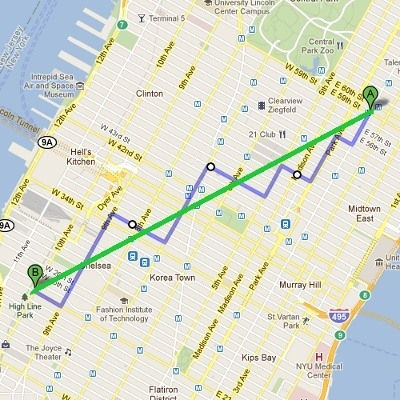
\includegraphics{MvsE}

		\subsubsection{Cosine Similarity}
			When documents are represented as term vectors, the sim- ilarity of two documents corresponds to the correlation be- tween the vectors. This is quantified as the cosine of the angle between vectors, that is, the so-called cosine similar- ity. Cosine similarity is one of the most popular similarity measure applied to text documents, such as in numerous in- formation retrieval applications [21] and clustering too [9].
			Given two documents t a and t b, their cosine similarity is
			\toadd{formule}
			where t a and t b are m-dimensional vectors over the term set T = {t 1,\ldots, t m }. Each dimension represents a term with its weight in the document, which is non-negative. As a result, the cosine similarity is non-negative and bounded between [0,1].
			An important property of the cosine similarity is its inde- pendence of document length. For example, combining two identical copies of a document d to get a new pseudo docu- ment d 0, the cosine similarity between d and d 0 is 1, which means that these two documents are regarded to be iden- tical. Meanwhile, given another document l, d and d 0 will have the same similarity value to l, that is, sim (t d, t l) = sim (t d 0, t l). In other words, documents with the same com- position but different totals will be treated identically. Strictly speaking, this does not satisfy the second condition of a met- ric, because after all the combination of two copies is a differ- ent object from the original document. However, in practice, when the term vectors are normalized to a unit length such as 1, and in this case the representation of d and d 0 is the same.
			\includegraphics{CvsE}

		\subsubsection{Jaccard Coefficient}
			The Jaccard coefficient, which is sometimes referred to as the Tanimoto coefficient, measures similarity as the intersection
			divided by the union of the objects. For text document, the Jaccard coefficient compares the sum weight of shared terms to the sum weight of terms that are present in either of the two document but are not the shared terms. The formal definition is:
			\toadd{formule}
			The Jaccard coefficient is a similarity measure and ranges between 0 and 1. It is 1 when the t a = t b and 0 when t a and t b are disjoint, where 1 means the two objects are the same and 0 means they are completely different. The corresponding distance measure is D J = 1 − SIM J and we will use D J instead in subsequent experiments.

		\subsubsection{Pearson Correlation Coefficient}
			Pearson’s correlation coefficient is another measure of the extent to which two vectors are related. There are different forms of the Pearson correlation coefficient formula. Given the term set T = {t 1,\ldots,t m }, a commonly used form is
			\toadd{formule}
			This is also a similarity measure. However, unlike the other measures, it ranges from +1 to −1 and it is 1 when t a = t b. In subsequent experiments we use the corresponding distance measure, which is D P = 1−SIM P when SIM P ≥ 0 and D P = |SIM P | when SIM P < 0.

		\subsubsection{Averaged Kullback-Leibler Divergence}
			In information theory based clustering, a document is con- sidered as a probability distribution of terms. The similarity of two documents is measured as the distance between the two corresponding probability distributions. The Kullback- Leibler divergence (KL divergence), also called the relative entropy, is a widely applied measure for evaluating the dif- ferences between two probability distributions.  
			Given two distributions P and Q, the KL divergence from distribution P to distribution Q is defined as
			\toadd{formule}
			In the document scenario, the divergence between two dis-
			tribution of words is:
			\toadd{formule}
			However, unlike the previous measures, the KL divergence is not symmetric, ie. D KL (P kQ) 6 = D KL (QkP). Therefore it is not a true metric. As a result, we use the averaged KL divergence instead, which is defined as
			\toadd{formule}
			The average weighting between two vectors ensures symme- try, that is, the divergence from document i to document j is the same as the divergence from document j to document i. The averaged KL divergence has recently been applied to clustering text documents, such as in the family of the Information Bottleneck clustering algorithms [18], to good effect.

		\subsubsection{Kiti}
		\begin{itemize}
			\item Manheteno
			\item Euklido
			\item Euklido atstumo kvadratas
			\item Čebyševo atstumas 
			\item Minkowski atstumas 
			\item Kosinuso atstumas 
			\item Žakardo atstumas 
			\item Daiso atstumas 
		\end{itemize}

	


	\subsection{Algoritmų skirstymas}


	\subsubsection{Algoritmų rūšys}
	\note{Kita skistymo versija}
	Duomenų klasterizavimo algroritmai bendrai gali būti suskirstyti į\cite{kadhim2014text}: 
	\begin{itemize}
		\item \ltang{\textbf{Padalijimo metodai}}{Partitioning methods}
		\item \ltang{\textbf{Herarkiniai metodai}}{Hierarchical methods}
		\item \ltang{\textbf{Tankumu paremti metodai}}{Density-based methods}
		\item \ltang{\textbf{Tinkliniai metodai}}{Grid-based methods}
		\item \ltang{\textbf{Modeliu paremti metodai}}{Model-based methods}
		\item \ltang{\textbf{Dažni struktūriniai metodai}}{Frequent pattern-based clustering}
		\item \ltang{\textbf{Suvaržymu paremti metodai}}{Constraint-based clustering}
		\item Papildomi, pritaikomi Web dokumentų klasterizacijai\cite{oikonomakou2005review} 
		\item \ltang{\textbf{Grafų metodai}}{Graph based clustering}
		\item \ltang{\textbf{Neuroninių tinklų metodai}}{Neural Network based clustering}
		\item \ltang{\textbf{Tikimybiniai metodai}}{Probabilistic clustering}
		\item \ltang{\textbf{Ontologiniai metodai}}{Ontological clustering}
		\item \ltang{\textbf{Nuorodomis paremti metodai}}{Link-based clustering}
	\end{itemize}

	Dar kiti suskirstymai rementis wikipedia
	\begin{itemize}
		\item Jungiantys modeliai: pavyzdžiui, hierarchinė klasterizacija nubraižo modelį remiantis jungčių atstumais.
		\item Centroidiniai modeliai: pavyzdžiui, k-vidurkių algoritmai aprašo kiekvieną klasterį vienu vektorių vidurkiu.
		\item Pasiskirstymo modeliai: klasteriai modeliuojami remiantis statistiniais pasiskirstymais, pavyzdžiui kelių kintamųjų normalinis pasiskirstymas naudojamas lūkesčių-maksimizavimo algoritmo.
		\item Tankio modeliai: pavyzdžiui, DBSCAN ir OPTICS aprašo klasterius kaip tankius regionus duomenų erdvėje.
		\item Poerdvių modeliai: Biklasterizacija (taip žinoma kaip Ko-klasterizacija, ar dviejų-tipų-klasterizacija), klasteriai yra modeliuojami naudojant klasterių narius ir reikšmingas savybes.
		\item Grupiniai modeliai: kai kurie algoritmai nesuteikia išdirbto modelio gautiems rezultatams ir pateikia tik tam tikrą grupinę informaciją.
		\item Grafais-paremti modeliai: klika (tam tikra grupė su panašiais parametrais), kuri yra dalinis mazgų rinkinys grafe taip sujungtų, kad du mazgai tarpusavyje yra sujungti paviršiumi, kuris laikomas prototipine klasterio forma. Tam tikrų jungčių atpalaidavimas yra vadinamas kvazi-klikomis HCS klasterizacijos algoritmas.
	\end{itemize}


	Padalinjimo metodai sugeneruoja nepersidengenčių duomeų \ltang{pogrupius}{subset} taip, kad kiekvienas duomuo yra tik viename pogrupyje. Šiems metodams reikia išanksto nurodyti kiek klasterių norima turėti. Keletas šio tipo technikų: k-means ir variacijos of k-means-bisecting, k-medoids, PAM (Kaufman and Rousseeuw, 1987), CLARA (Kaufmann and Rousseeuw, 1990), CLARANS (Ng and Han, 1994)\ldots

	Herarchiniai metodai sugenretuoja \ltang{}{nested} grupe klasterių kurie yra suskirstyti pagal medžio struktūrą. Šie algoritmai papildomai skirstomi į:\\
		\ltang{aglomeraciniai}{agglomerative} – dar kitaip žinomi kaip \ltang{iš apačios į viršų}{bottom-up} iš pradžių duomenis laiko kaip atskiras klasterio dalis ir nuosekliai jungia poras artimiausių klasterių į naujus tol kol visi klasteriai sujungiami į vieną.\\
		\ltang{diviziniai}{divisive} – dar kitaip žinomas kaip \ltang{iš viršaus į apačią}{top-down} iš pradžių visi duomenys priskiriami vienam klasteriu ir padalijimai yra atliekami rekursyviai besileidžian herarchija.Viešai prieinamos herarchinės technikos yra ROCK [4], Chamelon [5], BIRCH [6] and UPGMA.\needsource{išimk reikalingas citatas} \\
		Tankumo technikos sugrupuoja duomenis kurie yra pakankamai arti vieni kitų (tankūs), o retai išsidėsčiusius duomenis laiko \ltang{triukšmu}{noise} ir yra nepriskiremi jokiam klasteriui. Viešai prieinamos technikos yra DBSCAN ir praplėtimai, OPTICS and DENCLUE [6].\\
		Tinkliniai metodai naudoja \ltang{skirtingos raiškos}{multi\textendash{} resolution} tinklelio struktūrą duomenų surinkimui. Pagrindinis šios technikos privalumas \textendash{} našumas.\\
		Modelinės technikos gauna nurodumus kaip turi atrodyti klasteriai ir tada bando kiek galima geraiu joms pritaikyti duomenis.\\
		Dazniu paremti modeliai, as ju kolkas nesuprantu.\\
	Suvaržymų (reikalavimų) paremti metodai naudojasi vartotojo ar programos nurodytais reikalavimais.\toadd{better explenation}


	Klasteringo algoritmai skirstomi į šiuos tipus:
	\begin{itemize}
		\item \textbf{monothetic }– visi populiacijos nariai turi kažkokia bendrą savybę (vyrai nuo 20 iki 25 metų amžiaus)
			\\\textbf{polythetic }– nariai yra panšūs, bet neturi konkrečios bendros savybės (kai atstumas tarp narių nurodo priklausomybę grupei)
		\item \ltang{\textbf{kieti}}{hard} klasteriai – kai grupės neturi bendrų elementų. Kartais gali susidaryti atvėjai kai elementas “matematiškai” priklauso ne vienai grupei. Nortin išlaikyti determiniškumą tokiu atveju reikia nurodyti pasirinkimo taisykle.
			\\\ltang{\textbf{minkšti}}{soft} klasteriai – kai grupės gali turėti bendrų elementų. Tokiu atveju galime nagrinėti kaip konkretus elementas priklauso skirtingoms grupėms ir kaip gerai jas atitinka.
		\item \ltang{\textbf{plokšti}}{flat} – kai elementai suskirstomi į grupes, kurios viena kitai yra lygios.
			\\\ltang{\textbf{herarkiški}}{hierarchical} (taxonomy) – Kai grupė gali būti sudaryta iš kelių “konkretesnių” grupių. Pvz.\ retryveris $\,\to\,$ šuo $\,\to\,$ žinduolis $\,\to\,$ gyvūnas
	\end{itemize}
	Šiame skyriuje apžvelksiu algoritmų:

	\iffalse{}
	\begin{table}[H]\footnotesize
	\centering
	\caption{Lentelės pavyzdys}    % Antraštė įterpiama prieš lentelę
	{\begin{tabular}{lccc} 
		\toprule
		Algoritmas & \multicolumn{3}{c}{Tipas} \\
		\midrule
		%K-mean & hard & flat & polythetic \\ %\midrule
		%Hierarchical & hard & x & x\\
		\bottomrule
	\end{tabular}}
	\end{table}
	\fi{}
	\subsection{Centroidais paremta klasterizacija}
		\subsubsection{K-means}
			\ltang{K-vidurkių}{K-mean} algoritmas suskirsto duomenis į nurodytą ($ k $) klasterių. \[ \underset{\mathbf{S}} {\operatorname{\arg \min}}  \sum_{i=1}^{k} \sum_{\mathbf x \in S_i} \left\| \mathbf x - \boldsymbol\mu_i \right\|^2 \]
			Praktikoje dažniausiai naudojamas duodama $n$ vektroių (su $d$ dimensijų) ir numeris $k$.  Sustatome $k$ centroidų $c$ į atsitiktines vietas.
			\begin{enumerate}
				\item Kiekvienam taskui (vektoriui) randame artimiausia c
				\item Kiekviena centroida pakeiti taip kad jis geriau atitiktu jam priskirtą klusterį (sumažinti atstuma iki visų taškų arba kitaip tariant rasti taškų centrą). Tada eini i žingsni  1.\ %TODO add proper reference
				tol kol visi klusteriai išlieka vienodi.
			\end{enumerate}
			\BigO{iteracijos*K*n*d} produce hard, flat, polythetic cluster. 
		
		\subsubsection{fuzzy k-means}
			fuzzy k-means klasterizavimas yra vienas iš populiariausių klasterizavimo algoritmų k-means išplėtimas. k-means klasterizavimas suskirsto duomenis į atskiras grupes, kai vienas objektas gali priklausyti tik vienam klasteriui, tuo tarpu fuzzy k-means klasterizavimo algoritmas duomenis suskirsto į klasterius, kai objektas gali priklausyti skirtingoms grupėms (klasteriams) su tam tikra tikimybe.\\
			fuzzy k-means klasterizavimo algoritmo veikimas yra toks: kiekvieno aibės objekto priklausomybė bet kokiam klasteriui $k$ yra neapibrėžta. aibės objektai klasteriams priklauso su tikimybėmis $p(wi | xj, \theta)$, kur $\theta$ – duomenų vektorius priklausomybių funkcijoms. fuzzy k-means klasterizavimo algoritmas stengiasi sumažinti kainų funkciją jfuz:
			\begin{equation}
				jfuz=\sum{(\sum{(p(wi|xj,\theta)b‖xj−μi‖2)}nj=1)}ci = 1,
			\end{equation}
			kur kintamasis $b$ reguliuoja skirtingų klasterių persidengimą.\\
			visoms duomenų aibėms klasteriai turi sureguliuoti svorius, atsižvelgiant į pateiktų duomenų atstumus, bei klasterių svorius, kurie nusako tikimybes ar duomenų aibės priklauso pateiktiems klasteriams. fuzzy k-means klasterizavimo sudėtingumas:\BigO{ndc^2i}.
			\includegraphics{FKM}

		%\subsection{mixture models}
	\subsection{Jungianti klasterizacija (hierarchinė klasterizacija)}
		\ltang{Hierarchical}{Hierarchinis} klasterizavimo algoritmai yra viena iš populiariausių dokumentų klasterizavimo algoritmų grupė. Hierarchinis klasterizavimo algoritmas plačiai naudojamas iki šių dienų, nors šis algoritmas yra vienas iš pirmujų klasterizavimo algoritmų. Šis algoritmas labiausiai tinkamas naudoti klasterizuojant nedidelius duomenų rinkinius. Pradžioje hierarchinis algoritmas nustato bendrą visų klasterių tarpusavio priklausomybių struktūrą, ir tik tada sprendžia koks klasterių skaičius yra optimalus [11]. Hierarchinio klasterizavimo sudėtingumas: \BigO{n^3}.\\
		Hierarchinis klasterizavimo algoritmas skirstomas į du algoritmus: jungimo ir skaidymo.
		\begin{itemize}
			\item \ltang{Skaidymo}{divisive} algoritmas – pradinis klasteris susideda iš visos duomenų aibės ir nuosekliai dalinamas į smulkesnius klasterius.
			\item \ltang{Jungimo}{agglomerative} algoritmas – pradinis klasteris susideda iš vieno objekto ir prie jo jungiant kitus objektus (duomenis) gaunami vis didesni klasteriai, kol gaunamas vienas didelis klasteris.
		\end{itemize}
		\includegraphics{hierargram}
		Hierarchinio klasterizavimo algoritmo atstumai tarp klasterių skaičiuojami keliais metodais:
		\begin{itemize}
			\item \ltang{Artimiausias atstumas}{Single-link},
			\item \ltang{Tolimiausias atstumas}{Complete-link},
			\item Vidutinis atstumas,
			\item Centroidės atstumas,
			\item Ward atstumas – Euklido atstumo sumos kvadrato minimumas.
		\end{itemize}
		Šiuo metu populiariausiais laikomi 1 Artimiausio atstumo ir 2 Tolimiausio atstumo algoritmai.  Single-link algoritmas kuris dar žinomas kaip mažiausias skaičiuoja dviejų objektų atstumą kuris yra prilyginamas atstumui tarp dviejų artimiausių objektų. Complete-link algoritmas kuris žinomas kaip didžiausias skaičiuoja dviejų objektų atstumą, kuris yra prilyginamas atstumui tarp dviejų tolimiausių objektų.
	\subsection{Pasiskirstymu paremta klasterizacija}
		\subsubsection{EM}
			\ltang{em}{expectation maximization} algoritmas kitaip dar vadinamas tikimybinis klasterizavimo algoritmas.  tegul stebinys $x$ priklauso vienai iš $q$ skirtingų klasių, kur $v$ žymi stebimos klasės numerį $f_i(x)$ – sąlyginis pasiskirstymo tankis kai $v = i$. klasterizuojant tokią imtį daroma prielaida, kad $f_1,f_2,\ldots,f_q$ yra normaliniai pasiskirstymo tankiai su vidurkiais $m(i)$ ir kovariacinėmis matricomis $r(i)$.\\
			\begin{equation}
				f(x)=\sum^q_{i=1} {q_i f_i (x) = f(x, \theta)}
			\end{equation} 
			tada
			kur $\theta$ yra visų parametrų vektorius.\\
			klasterizavimas remiasi aposteriorinių tikimybių
			\begin{equation}
				\pi_i (x) = p\{v = i |x = x\} = \frac{p_i f_i(x)}{f(x,\theta)}
			\end{equation} 
			vertinimu\\
			$v(x) = argmaxi \pi_i(x)$\\
			em algoritmas yra rekurentinė procedūra, skirta $\theta$ maksimalaus tikėtinumo įverčio ir jį atitinkančių $\pi_i$ įverčių apskaičiavimui.
			\includegraphics{temp0}
			taigi, pasiskirstymo tankio funkcija $f(x)$ statistinį vertinimą, kai imtis yra klasterizuojama į $q$ klasterių $x = \{x(1), x(2), \ldots, x(n)\}$ siūloma atlikti dviem etapais:\\
			griežto klasterizavimo – kai $x = k_1\cup  \ldots \cup k_q$, kur kiekvienas $x(t)$ priklauso vienam ir tik vienam klasteriui $k_i$, kai $i = 1, 2, \ldots, q$.
			negriežto klasterizavimo – kai klasteriai $k_i$ suprantami kaip aibės $\{(x(1), \pi_i (1)), \ldots, (x(n), \pi_i(n))\}$, kur $\pi_i(t)$ rodo su kokiu svoriu (tikimybe) stebinys $x(t)$ priskiriamas klasei $k_i$. mišinio komponentai $f_i(x)$ vertinami pagal klasterio $k_i$ elementus, taikant vieną iš žinomų neparametrinio vertinimo metodų.
			\includegraphics{EM}

	\subsection{Tankiu-paremta klasterizacija}
		\subsubsection{dbsc}
			\toadd{koks skirtumas lyginant su dbscan}
			\ltang{dbsc}{density based spatial clustering} tai duomenų tankiu pagrįstas klasterizavimo metodas, kaimyninius duomenis grupuojantis į klasterius ne pagal atstumo matą, o pagal objektų tankį. tankis tai minimalus taškų atstumas, tarp kurių yra tam tikras atstumas. taškai, kurie nutolę tam tikru nustatytu atstumu vienas nuo kito, vadinami kaimynais. pagal tam tikrą tankio funkciją arba pagal kaimynystės tankį yra sudaromi klasteriai. sudėtingos struktūros klasterius sugeba atskirti tankiu grindžiami algoritmai. šie algoritmai taškų atsiskyrėlių neįtraukia į klasterius.
			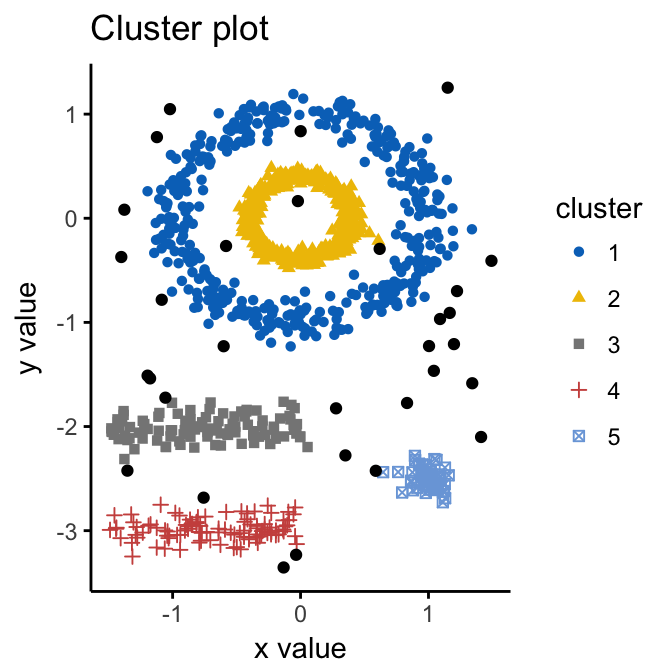
\includegraphics{DBSCAN}

	\subsection{Nzn konkrečios grupės}	

		\subsubsection{tolimiausio kaimyno}
			\ltang{tolimiausio kaimyno}{farthest first}klasterizavimo algoritmas, kuris visus duomenis skisto į klasterius palaipsniui – sukuria po vieną naują klasterį kiekvienoje iteracijoje. pirmuoju žingsniu visi duomenys priskiriami vienam klasteriui, tame klasteryje surandami du duomenys kurie labiausiai skiriasi vienas nuo kito. tuomet, pradinis klasteris išskaidomas į du naujus klasterius, kurių pradiniai duomenys skaidomojo klasterio labiausiai besiskiriantys duomenys. kol nepriskirti kiti duomenys, tol jie sutampa su išskaidytų klasterių centroidais. paskui likę duomenys priskiriami vienam iš naujai sukurtų dviejų klasterių. pirmoje iteracijoje pasirenkamas vienas klasteris, pagal tam tikrus kriterijus ir jis vėl skaidomas į du naujus klasterius. kriterijai gali būti įvairūs – klasterio dydis, maksimalus klasterio diametras, ir pns. klasterių skaidymas vykdomas tol, kol gaunamas reikiamas kiekis klasterių.\\
			\includegraphics{FF}

		\subsubsection{Dirichlet}
			dirichlet klasterizavimas yra $p$ vektorių tikimybių pasiskirstymo funkcija. visi vektoriai $p$ atspindi duomenų pasiskirstymo tikimybes $a$. dirichlet klasterizavimas apibrėžiamas vektoriumi $ \alpha = {\alpha i}i=1|a+|$, kai $ \alpha i > 0$,\\
			\begin{equation}
				(p|\alpha)=\gamma(|\alpha|)\pi i=1|a|\gamma (\alpha i)\pi i=1|a|pi \alpha i−1,
			\end{equation}
			čia $\pi$ (.) žymi – gama funkciją, $\sum{pi=1|a|i=1}$, bei $|\alpha| = \sum{\alpha i|a|i=1,pi≥0} (i =1,\ldots,|a|)$.
			dirichlet klasterizavimas paremtas individualių klasterių matematine kombinacija, kuri naujai sukuria tikimybių pasiskirstymą. visiems skirtingiems klasteriams suteikiami svoriai, jie vadinami koeficientais. klasterių paskirstymas $\varphi$, kuris sudarytas iš $l$ komponentų, gaunamas iš:
			\begin{equation}
				\varphi = \sum{qjgjlj=1},
			\end{equation}
			$gj$ – yra dirichlet klasteriai. kiekvienas klasteris aprašo pasiskirstymo dėsnį. duomenų skaičius klasteriuose yra neribojamas, tačiau naudojant didelį kiekį duomenų šis metodas veikia neoptimaliai.

	\subsection{Kiti metodai}
			Taip pat yra medodų kuriuos būtu galima priskirti kelioms rušims, ar ne neivienai. 
		\subsubsection{Dalinai prižiūrimas klasterizavimas}
			Semi-supervised clustering
		\subsubsection{Mišrus klasterizavimas}
			Mixed clustering

	\subsection{Su klasterizavimu susiję metodai}

		\subsubsection{latent dirichlet allocation}
			latent dirichlet allocation (toliau lda, nesumaišyti su linear discriminant analysis, kas yra kitas mašininio mokymosi metodas). yra kurkas sudetingesnis dokumentu analizavimo metodas. kartais priskiremas atskirai algoritmu klasei topic modeling, kuri bando ne grupuoti duomenis o suteigti jiems temas. palyginant su praeitais metodais dokumentai turėjo priklausyti vienai iš klasterių ar jų herarkijai, bet dokumentas gali turėti kelias temas. 
			% reikia perkelti ir tiksliau apibrėžti ką būtent gražina.	
			todėl lda gražina ne sugrupuotus duomenis, o pasiskirstymą kiek kokių temų turi kiekvienas dokumentas  

\section{Algoritmų testavimas/kokybės vertinimas}
	\toadd{purity and entropy}
	viena iš fundamentalių neprižiūrimo mokymosi problemų yra modelių testavimas. skirtingai nei „prižurimame mokymasi“ kur svarbu atdidėti dali duomenų su kuriais nėra mokomasi o tik testuojama sugeneruoti modeliai, „neprižiurimame mokymasi“ mes to nelgalim atlikti\ldots bet egzsituoja keltatas metodu kaip galima patikrinti sudarytus klasterius.
	\begin{itemize}
		\item pirma galima sugeneruotus klasterius leisti tikrinti \textbf{žmonėms }. tam yra keli būdai. galima tiesiog duoti sugeneruotus klasterius ir bandyti nuspresti ar jie tinkami. taipat galima parainkti du atsitiktinius dokumentus ir spėti ar jie turėtu būti viename ar atskiruose klasteriuose, ir tada palyginti su kompiuterio sugeneruotu rezultatu. 
		\item taip yra metodų kaip atlikti testavimą automatiškai. vienas jų paimti 2(ar daugiau) dokumentus iš skirtingų klasterių ir apkeisti juos vietomis, tada patikrinti klasteriu //stipruma. tai atlike dokybe kartų galime spręsti kaip sėkmingai sekėsi klasterizacija, jeigu apmainant jų kokybė nukrito tai reikškia, kad dokumentai sėkmingai suklaserizuoti, bet jeigu nesikeite tai reiške, kad klasteriai mažai vienas nuo kito skiresi ir klasreizacija nesekminga.
	\end{itemize}

\sectionnonum{Išvados}
	%išvadose ir pasiūlymuose, nekartojant atskirų dalių apibendrinimų, suformuluojamos svarbiausios darbo išvados, rekomendacijos bei pasiūlymai.


\printbibliography[heading=bibintoc] % literatūros šaltiniai aprašomi
% bibliografija.bib faile. šaltinių sąraše nurodoma panaudota literatūra,
% kitokie šaltiniai. abėcėlės tvarka išdėstoma tik darbe panaudotų (cituotų,
% perfrazuotų ar bent paminėtų) mokslo leidinių, kitokių publikacijų
% bibliografiniai aprašai (šiuo punktu pasirūpina latex). aprašai pateikiami
% netransliteruoti.

\appendix  % Priedai
% Prieduose gali būti pateikiama pagalbinė, ypač darbo autoriaus savarankiškai
% parengta, medžiaga. Savarankiški priedai gali būti pateikiami kompiuterio
% diskelyje ar kompaktiniame diske. Priedai taip pat vadinami ir numeruojami.
% Tekstas su priedais siejamas nuorodomis (pvz.: \ref{img:mlp}).

\end{document}
